% Partial sums of e(n/5). Vertices computed from the fifth roots of unity; S_5=0.
\begin{tikzpicture}[every node/.style={font=\footnotesize},scale=1.15]
  \draw[MidnightBlue,thick] (0,0)--(0.309,0.951)--(-0.500,1.539)--(-1.309,0.951)--(-1,0)--(0,0);
  \fill[BurntOrange] (0,0) circle (1.5pt);
  \fill[MidnightBlue] (0.309,0.951) circle (1.2pt);
  \fill[MidnightBlue] (-0.500,1.539) circle (1.2pt);
  \fill[MidnightBlue] (-1.309,0.951) circle (1.2pt);
  \fill[MidnightBlue] (-1,0) circle (1.2pt);
  \node[below right] at (0.05,-0.02) {$S_0=0$};
  \node[right] at (0.35,0.95) {$S_1$};
  \node[above] at (-0.50,1.58) {$S_2$};
  \node[left] at (-1.35,0.95) {$S_3$};
  \node[below] at (-1,-0.02) {$S_4=-1$};
  \node at (1.55,0.75) {$\alpha=\dfrac{1}{5}$};
\end{tikzpicture}
